\anonsection{Задание 7}
\anonsubsection{Формулировка задания}

\begin{enumerate}
	\item Методом случайного поиска найти минимальное значение функции
     $f$ на множестве $A = \{x_1, x_2 : x_1^2 + x_2^2 \leq 1\}$, т.е.
     $y = \min f(x)$, где 
\begin{equation}
    f(x) = x_1^3 \sin \left( \frac{1}{x_1} \right) + 10 x_1 x_2^4 \cos 
     \left( \frac{1}{x_2} \right)
\end{equation}
     при $ x_1 \neq 0 $ и $ x_2 \neq 0 $, функция доопределяется по
     непрерывности при $ x_1 = 0 $ или $ x_2 = 0 $.
    \item Методом имитации отжига найти минимальное значение функции
     Розенброка $ g $ в пространстве $ \mathbb{R}^2 $, где 
\begin{center}
	$ g(x) = (x_1 - 1)^2 + 100 (x_2 - x_1^2)^2 $
\end{center}
    \item Оценить точность. Сравнить результаты со стандартными методами
     оптимизации.
\end{enumerate}

\anonsubsection{Метод случайного поиска}
Возьмем единичный круг и сгенерируем на нём набор равномерно распределенных
 по нему точек. Найдем миниммальное значение.\\
Совместная плотность равномерного распределения случайных величин $ x_1,
 x_2 $ на единичном круге равна:
\begin{equation}
    f_{x_1, x_2} = \begin{cases}
        \frac{1}{\pi}, & x_1^2 + x_2^2 \leq 1,\\
        0, &\text{иначе.}
    \end{cases}
\end{equation}
В полярных координатах:
\begin{equation}
    \left\{
    \begin{array}{lll}
        x_1 = r\cos\varphi, &0 \leqslant r \leqslant 1,\\
        x_2 = r\sin\varphi, &0 \leqslant\varphi\leqslant 2\pi.\\
    \end{array}
    \right.
\end{equation}
Таким образом, получим:
\begin{equation} \label{p81}
    \mathbb{P}((x_1, x_2) \in A) = \iint \limits_{x_1^2 + x_2^2 \leq 1} 
     \frac{1}{\pi} dx_1 dx_2 = \frac{1}{\pi} \int\limits_0^1 r dr 
     \int\limits_0^{2\pi} d\varphi = \int\limits_0^1 dr^2 \int\limits_0^{2\pi}
     \frac{1}{2\pi} d\varphi.
\end{equation}
Сделаем замену
\begin{equation*}
q = r^2,\;r = \sqrt{q},\;q\in[0, 1].
\end{equation*}
Тогда выражение в \eqref{p81} примет вид:
\begin{equation}
\mathbb{P}((x_1, x_2)\in A) = \int\limits_0^1 dq\int\limits_0^{2\pi}
 \frac{1}{2\pi}d\varphi.
\end{equation}
Следовательно, $x_1$ и $x_2$ выражаются в виде:
\begin{equation*}
\left\{
\begin{array}{lll}
x_1 = \sqrt{q}\cos\varphi, &q\sim U[0, 1],\\
x_2 = \sqrt{q}\sin\varphi, &\varphi\sim U[0, 2\pi].\\
\end{array}
\right.
\end{equation*}
Отметим, что данная функция имеет минимум на границе единичного круга,
 поэтому поиск можно сократить, генерируя случаные точки исключительно
 на границе области. На Рис. \eqref{fig:random_min} изображен график функции
 и отмечена найденная с помощью алгоритма точка минимума.

\begin{figure}[ht]
	\centering
	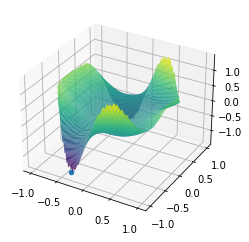
\includegraphics[width = 0.5\linewidth]{"./resources/random_min.png"}
	\caption{Минимум функции, найденный с помощью алгоритма случайного 
     поиска: \( x_{min} = -0.360171, y_{min} = 0.146528, f_{min} = -1.288383. \)}
    \label{fig:random_min}
\end{figure}

\anonsubsection{Метод имитации отжига}

Алгоритм основывается на имитации физического процесса, который происходит
 при кристаллизации вещества, в том числе при отжиге металлов. Предполагается,
 что атомы уже выстроились в кристалличекую решётку, но ещё допустимы переходы
 отдельных атомов из одной ячейки в другую. Предполагается, что процесс
 протекает при постепенно понижающейся температуре. Переход атома из одной 
 ячейки в другую происходит с некоторой вероятностью, причём вероятность 
 понижается с понижением температуры. Устойчивая кристаллическая решётка 
 соответствует минимуму энергии атомов, поэтому атом либо переходит в 
 состояние с меньшим уровнем энергии, либо остаётся на месте.

При помощи моделирования такого процесса ищется такая точка или множество 
 точек, на котором достигается минимум некоторой числовой функции 
 \( F(\overline{x}) \), где \( \overline{x}=(x_{1}, \dots,x_{m}) \in X \).
 Решение ищется последовательным вычислением точек \( \overline{x_0}, 
 \overline{x_1}, \dots, \) пространства \( X \); каждая точка, начиная с
 \( \overline{x_{1}} \), "<претендует"> на то, чтобы лучше предыдущих
 приближать решение. Алгоритм принимает точку \( \overline{x_{0}} \) как 
 исходные данные. На каждом шаге алгоритм (который описан ниже) вычисляет 
 новую точку и понижает значение величины (изначально положительной), 
 понимаемой как "<температура">. Алгоритм останавливается по достижении 
 точки, которая оказывается при температуре ноль.

Точка \( \overline{x_{i+1}} \) по алгоритму получается на основе текущей 
 точки \( \overline{x_{i}} \) следующим образом. К точке \( \overline{x_i}
 \) применяется оператор \( A \), который случайным образом модифицирует 
 соответствующую точку, в результате чего получается новая точка 
 \( \overline{x^*} \). Точка \( \overline{x^*} \) становится точкой 
 \( \overline{x_{i+1}} \) с вероятностью \( P \left( \overline{x^*}, 
 \overline{x_{i+1}} \right) \), которая вычисляется в соответствии с 
 распределением Гиббса:
\[
 P \left( \overline{x^*} \to \overline{x_{i+1}} | \overline{x_{i}} \right) 
 = \begin{cases} 
    1, & F( \overline{x^{*}} ) -F( \overline{x_{i}}) < 0,\\
    \exp \left( -\dfrac{F(\overline{x^{*}}) - F(\overline{x_{i}})}{T_i}
    \right), & F(\overline{x^{*}}) - F(\overline{x_{i}}) \geq 0.
 \end{cases}
\]

Здесь \( T_i>0 \)~---~элементы произвольной убывающей, сходящейся к нулю
 положительной последовательности, которая задаёт аналог падающей 
 температуры в кристалле. Скорость убывания и закон убывания могут быть 
 заданы по желанию создателя алгоритма.

Алгоритм имитации отжига похож на градиентный спуск, но за счёт случайности
 выбора промежуточной точки должен попадать в локальные минимумы реже, чем 
 градиентный спуск. Алгоритм имитации отжига не гарантирует нахождения 
 минимума функции, однако при правильной политике генерации случайной 
 точки в пространстве \( X \), как правило, происходит улучшение начального 
 приближения.

На Рис.\eqref{fig:sim_annealing} показан результат работы алгоритма, 
 включая промежуточные точки, в которых он оказывается.

\begin{figure}[ht]
	\centering
	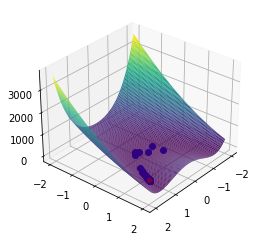
\includegraphics[width = 0.5\linewidth]{"./resources/sim_annealing.png"}
	\caption{Минимум функции, найденный с помощью алгоритма имитации отжига:
     \( x_{min} = 1.14533279, y_{min} = 1.31234433, f_{min} = 0.02115266.\)}
    \label{fig:sim_annealing}
\end{figure}

\anonsubsection{Оценка точности вычислений}
Пусть $x = (x_1, x_2)$ --- фактическая точка минимума, $\hat{x} = 
 (\hat{x}_1, \hat{x}_2)$ --- точка минимума, полученная методом случайного 
 поиска. Оценим $|x - \hat{x}|$.
Рассмотрим график исследуемой функции.

Исследуемая функция чётная по $x_1, x_2$, имеет несколько точек минимума, 
 которые не являются граничными. Тогда
\begin{equation*}
    |x - \hat{x}| \leq \varepsilon = \sqrt{\frac{p}{n}}.
\end{equation*}
Оценим $|f(x) - f(\hat{x})|$ через $|x - \hat{x}|$.\\
Поскольку $f$ --- непрерывна, то $f$ --- липшицева, следовательно:
\begin{equation*}
|f(a) - f(b)| \leq ||\nabla f||_\infty |a - b| = \underset{a, b\in A}{\esssup}
 |\nabla f| |a - b| = \max_{a, b \in A}|\nabla f| |a - b|, \forall a, b 
 \in A.
\end{equation*}
Оценим $\max\limits_{x_1, x_2 \in A} |\nabla f|$.\\
\begin{equation*}
\left|\frac{\partial f}{\partial x_1}\right| = \left|3x_1^2\sin(\frac{1}
 {x_1}) - x_1\cos(\frac{1}{x_1})+10x_2^4\cos(\frac{1}{x_2}) \right| \leq 
 3x_1^2+|x_1| +10x_2^4 \leq \sqrt{10} + 10,
\end{equation*}
\begin{equation*}
\left|\frac{\partial f}{\partial x_2}\right| = \left| 40x_1x_2^2 
 \cos(\frac{1}{x_2}) - 10x_1x_2^4 \cos(\frac{1}{x_2})\right| \leq 
 40|x_1|x_2^2 + 10|x_1|x_2^4 \leq 10\sqrt{17}.
\end{equation*}
Следовательно, $|\nabla f| = \sqrt{\left(\frac{\partial f}{\partial x_1} 
 \right)^2 + \left(\frac{\partial f}{\partial x_2}\right)} = 
 \sqrt{(\sqrt{10} + 10)^2+(10\sqrt{17})^2}\leq  34.26.$\\
Окончательная оценка точности вычислений:
\begin{equation*}
|f(x) - f(\hat{x})| \leq 34.26\sqrt{\frac{p}{n}}.
\end{equation*}